% !TEX root = ../waves.tex
%%%%%%%%%%%%%%%%%%%%%%%%%%%%%%%%%%%%%%%%%%%%%%%%%%%%%%%%%%%%%%%%%%%%%%%%%%%%%%%%%%%%%%%%%%
\section{General properties of periodic functions}
A physical quantity $f(t)$ depending on a variable $t$ is said to be \emph{oscillating} or
\emph{periodic} if it repeats itself identically after a certain duration. In mathematical
terms:
\begin{definition}
  A function $f(t)$ is said to be~\emph{periodic} if there exists $T>0$ such that
  \begin{equation}
    \forall t,\quad f(t+T)=f(t)\,.
  \end{equation}
  $T$ is called a \emph{period} of $f(t)$.
\end{definition}
\noindent For example, $\sin(t)$ is periodic with period $2\pi$, and a constant function
admit any number has a period. Another fundamental quantity is the \emph{frequency}:
\begin{definition}
  If $T$ is a period of a given periodic function $f(t)$, its inverse
  \begin{equation}
    \omega=\frac{1}{T}
  \end{equation}
  is called a \emph{frequency} of $f(t)$.
\end{definition}
\noindent In physical terms, if $t$ is a time variable, $T$ is also a time, and $\omega$
is the number of oscillations per unit of time. One can notice that a periodic function
never has a unique period, \eg clearly if $T$ is a period, $2T$ is also a period. Because
of this it is useful to write the following definition
\begin{definition}
  The infimum $T_0$ of the set of all possible periods of a given periodic function $f(t)$
  is called the \emph{fundamental period} of $f(t)$. The associated frequency
  $\omega_0=\frac{1}{T_0}$ is called the \emph{fundamental frequency} of $f(t)$.
\end{definition}
\noindent For example, the fundamental frequency of $\sin(t)$ is $2\pi$, and it is zero
for a constant function. Another fundamental quantity is the \emph{amplitude} of a
periodic function, measuring the size of the oscillations within a fundamental period:
\begin{definition}
  \label{def:amplitude}
  Let $f(t)$ be a real periodic function with fundamental period $T_0$. We additionally
  assume that $f(t)$ is bounded with infimum and supremum
  \begin{equation}
    m=\inf_{0\leq t\leq T_0}f(t)\qquad\text{and}\qquad M=\sup_{0\leq t\leq T_0}f(t)\,.
  \end{equation}
  The \emph{amplitude} of $f(t)$ is then defined by
  \begin{equation}
    A=\frac{M-m}{2}\,.
  \end{equation}
\end{definition}
\noindent For example, the amplitude of $\sin(t)$ is equal to $1$, and it is zero for
constant functions. \cref{def:amplitude} assumes that $f(t)$ is bounded, and one can
question whether this hypothesis is true in general. It is not, but continuity is a
sufficient condition:
\begin{proposition}
  If a real periodic function is continuous, then it is bounded (and therefore it has a
  well-defined amplitude).
\end{proposition}
\begin{proof}
  Let $f(t)$ be a continuous periodic function with fundamental period $T_0$. Since $f(t)$
  is continuous on the compact interval $[0,T_0]$, it follows from the boundedness theorem
  that it is also bounded on this interval. Finally, using the periodicity, any value
  $f(t)$ is equal to a value $f(t_0)$ with $0\leq t_0\leq T$, therefore $f(t)$ is bounded.
\end{proof}
\noindent One can show that this condition is not necessary, \ie discontinuous periodic
functions can be bounded as well. One example of such function is the \emph{square wave},
that will be useful later:
\begin{definition}
  \label{def:sq-wave}
  The square wave function $\sq(t)$ is defined by
  \begin{equation}
    \sq(t)=
    \begin{cases}
      1, &\text{if~}\lfloor 2t\rfloor~\text{is even}\\
      -1, &\text{if~}\lfloor 2t\rfloor~\text{is odd}\\
    \end{cases}\,,
  \end{equation}
  where $\lfloor t\rfloor$ is the floor function, \ie the largest integer smaller or equal
  to $t$.
\end{definition}
\noindent It is left as an exercise to the reader to show that $\sq(t)$ is periodic with
fundamental period $1$ and amplitude $1$, and can be rewritten as
\begin{equation}
  \sq(t)=2(2\lfloor t\rfloor-\lfloor 2t\rfloor)+1\,.
\end{equation}
Additionally, $\sq(t)$ is discontinuous at all points of the form $\frac{n}{2}$ where
$n\in\mathbb{Z}$. The curve of $\sq(t)$ is represented in~\cref{fig:sq-wave}.
\begin{figure}[t]
  \centering
  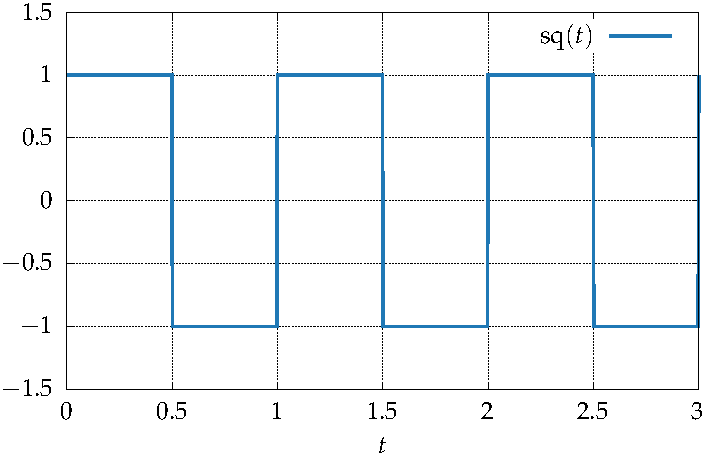
\includegraphics{gp_sq-wave.pdf}
  \caption{Curve of the square wave defined in~\cref{def:sq-wave}.}
  \label{fig:sq-wave}
\end{figure}
As mentioned above, the sine function provides a way to construct explicit examples of
periodic functions. We will see that it is, in fact, a fundamental building block of
periodic functions, which is the essence of Fourier analysis. It is therefore useful to
familiarise beforehand with periodic functions built using the sine function.
%%%%%%%%%%%%%%%%%%%%%%%%%%%%%%%%%%%%%%%%%%%%%%%%%%%%%%%%%%%%%%%%%%%%%%%%%%%%%%%%%%%%%%%%%%
\section{Elementary waves}
We start by defining elementary sine waves
\begin{definition}
  We call \emph{elementary sine wave} the function defined by
  \begin{equation}
    \sw(t;\omega,\phi)=\sin(2\pi\omega t + \phi)\,.\label{eq:sine-wave}
  \end{equation}
  where $\omega\geq 0$ and $0\leq\phi<2\pi$ are the \emph{frequency} and \emph{phase} of
  the wave, respectively. When the phase argument is omitted then it is assumed that
  $\phi=0$, \ie $\sw(t;\omega)=\sw(t;\omega,0)$.
\end{definition}
\noindent It is straightforward to show that, according to the definition in the previous
section, $\sw(t;\omega,\phi)$ is a periodic function with fundamental frequency $\omega$
and amplitude $1$. The phase measures the delay in the oscillation relatively to a wave
with identical frequency equal to zero at $t=0$. More generally if two waves have
identical frequencies and different phases $\phi_1$ and $\phi_2$, the time delay between
them is given by
\begin{equation}
  \delta t =\frac{T}{2\pi}\delta\phi\qquad\text{with}\qquad\delta\phi=\phi_1-\phi_2\,,
\end{equation}
explicitly
\begin{equation}
  \sw(t;\omega,\phi_1)=\sw(t+\delta t;\omega,\phi_2)\,.
\end{equation}
In other words, the phase can always be re-written as a shift in time:
\begin{equation}
  \sw(t;\omega,\phi)=\sw(t+t_0;\omega),
  \qquad\text{with}\qquad
  t_0 = \frac{T\phi}{2\pi}\,.\label{eq:phase-delay}
\end{equation}
The frequency and phase are represented graphically in~\cref{fig:sine-wave}.
\begin{figure}[t]
  \centering
  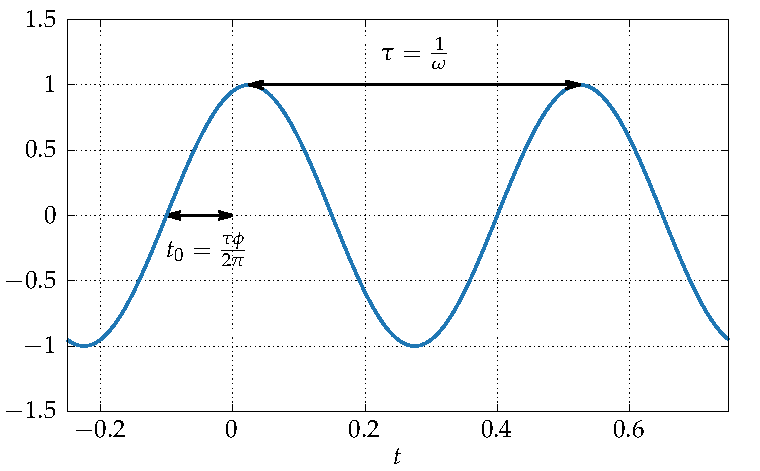
\includegraphics{gp_sine-wave.pdf}
  \caption{Example curve of the sine wave defined in~\cref{eq:sine-wave}, with frequency
    $\omega=2$ and phase $\phi=0.2\times 2\pi$. The arrows represent the period
  $T=\frac{1}{\omega}$ and the phase delay from~\cref{eq:phase-delay}.}
  \label{fig:sine-wave}
\end{figure}

For the special phase $\frac{\pi}{2}$, a sine wave can be written using the cosine
function:
\begin{equation}
  \sw\left(t;\omega,\frac{\pi}{2}\right)= \cos(2\pi\omega t)\,,
\end{equation}
motivating the following definition
\begin{definition}
  We call \emph{elementary cosine wave} the function
  \begin{equation}
    \cw(t;\omega,\phi)=\cos(2\pi\omega t + \phi)\,.\label{eq:cosine-wave}
  \end{equation}
  Similarly to the case of sine waves we define $\cw(t;\omega)=\cw(t;\omega,0)$. Sine and
  cosine waves are related by the following trivial relationships
  \begin{equation}
    \sw(t;\omega,\phi)=\cw\left(t;\omega,\phi-\frac{\pi}{2}\right),
    \quad\text{and}\quad
    \cw(t;\omega,\phi)=\sw\left(t;\omega,\phi+\frac{\pi}{2}\right)\,.
  \end{equation}
\end{definition}

A crucial set of formula to manipulate waves is given by the following angle addition
theorem:
\begin{theorem}[Angle addition]
  \label{thm:angle-add}
  For all pairs of real numbers $a$ and $b$, one has the following identities
  \begin{align}
    \sin(a+b)&=\sin(a)\cos(b)+\cos(a)\sin(b)\,,\label{eq:sinapb}\\
    \sin(a-b)&=\sin(a)\cos(b)-\cos(a)\sin(b)\,,\label{eq:sinamb}\\
    \cos(a+b)&=\cos(a)\cos(b)-\sin(a)\sin(b)\,,\label{eq:cosapb}\\
    \cos(a-b)&=\cos(a)\cos(b)+\sin(a)\sin(b)\,.\label{eq:cosamb}
  \end{align}
\end{theorem}
\begin{proof}
  We remind that the sine and cosine function are the real and imaginary part of complex
  exponential
  \begin{equation}
    e^{i\theta}=\cos(\theta)+i\sin(\theta)\,.
  \end{equation}
  Therefore,
  \begin{equation}
    e^{i a}e^{i b}=\cos(a)\cos(b)-\sin(a)\sin(b)+i[\cos(a)\sin(b)+\sin(a)\cos(b)]\,,\label{eq:eaeb}
  \end{equation}
  and by definition
  \begin{equation}
    e^{i(a+b)}=\cos(a+b)+i\sin(a+b)\,.\label{eq:eapb}
  \end{equation}
  Now, using the fact that $e^{i(a+b)}=e^{i a}e^{i b}$, and identifying the real and
  imaginary parts in~\cref{eq:eaeb,eq:eapb}, one directly
  obtains~\cref{eq:sinapb,eq:cosapb}. \cref{eq:sinamb,eq:cosamb} can then be obtained
  using the parity properties of the sine and cosine functions, namely $\sin(-x)=-\sin(x)$
  and $\cos(-x)=\cos(x)$.
\end{proof}
The angle addition theorem can be proven solely using triangle geometry, which is
significantly less trivial than the simple proof above based on complex numbers. More
generally, elementary waves are indeed easier to manipulate using complex exponentials,
motivating the definition below.
\begin{definition}
  We call \emph{elementary complex wave} the function
  \begin{equation}
    \ew(t;\omega,\phi)=e^{i(2\pi\omega t + \phi)}\,.
  \end{equation}
  As previously we define $\ew(t;\omega)=\ew(t;\omega,0)$. By definition of the complex
  exponential, elementary complex waves are related to sine and cosine elementary waves by
  the relation
  \begin{equation}
    \ew(t;\omega,\phi)=\cw(t;\omega,\phi)+i\,\sw(t;\omega,\phi)\,,
  \end{equation}
  Thanks to the properties of the exponential, we have the two following trivial
  relationships
  \begin{equation}
    \ew(t;\omega,\phi)=e^{i\phi}\ew(t;\omega)\,\quad\text{and}\quad
    \ew(t;\omega,\phi)^*=\ew(-t;\omega,-\phi)=\ew(t;-\omega,-\phi)\,,\label{eq:cw-conj}
  \end{equation}
  where $z^*$ is the conjugate of the complex number $z$. Using these formulas, the
  relationship to sine and cosine waves can be rewritten as
  \begin{align}
    \cw(t;\omega,\phi)&=\frac{1}{2}[\ew(t;\omega,\phi)+\ew(t;-\omega,-\phi)]\,,
    \label{eq:cwtoew}\\
    \sw(t;\omega,\phi)&=-\frac{i}{2}[\ew(t;\omega,\phi)-\ew(t;-\omega,-\phi)]\,.
    \label{eq:swtoew}
  \end{align}
\end{definition}

A considerable simplification with complex waves comes from the fact that the phase is
just a multiplicative factor, equivalent to giving a \emph{complex amplitude} to the wave.
Similarly, phased sine and cosine waves can be expressed as a sum of zero-phase ones using
the angle addition theorem:
\begin{align}
  \sw(t;\omega,\phi)&=\cos(\phi)\sw(t;\omega)+\sin(\phi)\cw(t;\omega)\,,\\
  \cw(t;\omega,\phi)&=\cos(\phi)\cw(t;\omega)-\sin(\phi)\sw(t;\omega)\,.
\end{align}
%%%%%%%%%%%%%%%%%%%%%%%%%%%%%%%%%%%%%%%%%%%%%%%%%%%%%%%%%%%%%%%%%%%%%%%%%%%%%%%%%%%%%%%%%%
\section{Combination of elementary waves}
We will now discuss how to create more general waves by adding elementary waves. One first
legitimate question is whether the sum of two periodic functions is till periodic. It is
not always true, and can be characterised by the following result:
\begin{theorem}
  \label{thm:period-sum}
  Let $f_1(t)$ and $f_2(t)$ be two periodic functions of fundamental periods $T_1\neq 0$
  and $T_2\neq 0$, respectively. Then, for any pair of non-zero complex numbers $\alpha_1$
  and $\alpha_2$, the linear combination
  \begin{equation}
    f(t)=\alpha_1 f_1(t)+\alpha_2 f_2(t)
  \end{equation}
  is periodic if and only if the period ratio  $\frac{T_1}{T_2}$ is a rational number. If
  this condition is true, this ratio can be written $\frac{T_1}{T_2}=\frac{p}{q}$ where
  $p$ and $q$ are two coprime integers (\ie their GCD is $1$), and the fundamental
  frequency $T$ of $f(t)$ is given by
  \begin{equation}
    T=qT_1=pT_2\,.
  \end{equation}
\end{theorem}
\begin{example}
  \label{ex:period-sum}
  $\sin\left(\frac{2\pi}{3}t\right)+\sin(\pi t)$ is periodic with fundamental period $6$.
\end{example}
\begin{example}
  \label{ex:nperiod-sum}
  $\sin(t)+\sin(\pi t)$ is not periodic.
\end{example}
\noindent Both examples above are illustrated in~\cref{fig:sine-sum}. Mathematically
speaking,~\cref{thm:period-sum} means that generally periodic functions sums are not
periodic. However, we remind that any real number is arbitrarily close to a rational
number, so non-periodic sums like in~\cref{ex:nperiod-sum} can always be approximated
arbitrarily well by a periodic function. This is relevant for physics and engineering
applications where quantities are often known up to some limited precision.
\begin{figure}[t]
  \centering
  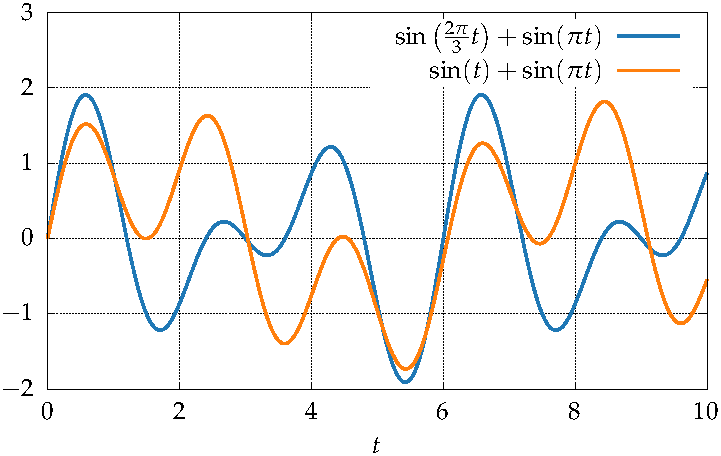
\includegraphics{gp_sine-sum.pdf}
  \caption{Curves of the sine wave sums in~\cref{ex:period-sum,ex:nperiod-sum}}
  \label{fig:sine-sum}
\end{figure}

%%%%%%%%%%%%%%%%%%%%%%%%%%%%%%%%%%%%%%%%%%%%%%%%%%%%%%%%%%%%%%%%%%%%%%%%%%%%%%%%%%%%%%%%%%
\section{Trigonometric polynomials}
We can make the following definition for an arbitrary linear
combination of elementary waves:
\begin{definition}
  We call \emph{trigonometric polynomial} of degree $N$ and frequency $\omega$ any
  function of the form
  \begin{equation}
    P(t)=a_0+\sum_{n=1}^N[a_n\,\cw(t;n\omega)+b_n\,\sw(t;n\omega)]\,,
    \label{eq:trigp-sc}
  \end{equation}
  where $a_n$ and $b_n$ are real coefficients such that $a_N\neq 0$ or $b_N \neq 0$. The
  formula above is called the \emph{sine-cosine form} of $P(t)$ with \emph{sine-cosine
  coefficients} or \emph{modes} $a_n$ and $b_n$.
\end{definition}
It is clear that such function is periodic, and a consequence of~\cref{thm:period-sum} is
then
\begin{proposition}
  Let $P$ be a trigonometric polynomial of degree $N\geq 1$ and frequency $\omega$ with
  sine-cosine coefficients $a_n$ and $b_n$. $P$ is a periodic function with period
  $T=\frac{1}{\omega}$, and additionally if $a_1\neq0$ or $b_1\neq0$, then $\omega$ is the
  fundamental frequency of $P(t)$.
\end{proposition}
\begin{proof}
  Each term in~\cref{eq:trigp-sc} is trivially $T$-periodic, so $P$ is also $T$-periodic.
  Now, the $n$-th mode of $P$ has a fundamental period of $T_n=\frac{T}{n}$. Assuming that
  $a_1\neq0$ or $b_1\neq0$, then the period ratio of this first mode to an arbitrary
  non-vanishing higher mode $n$ is given by
  \begin{equation}
    \frac{T_1}{T_n}=n\,.
  \end{equation}
  Using~\cref{thm:period-sum}, this means that this combination of modes has fundamental
  period $T$. The remaining modes can then be added one after another, and repeated use
  of~\cref{thm:period-sum} demonstrate the proposition.
\end{proof}
As we previously did for the elementary waves, trigonometric polynomials can be put in a
more convenient complex form
\begin{definition}
  \label{def:trigp-complex}
  Let $P$ be a trigonometric polynomial of degree $N$ and frequency $\omega$ with
  sine-cosine coefficients $a_n$ and $b_n$. $P$ can be written in the \emph{complex form}
  \begin{equation}
    P(t)=\sum_{n=-N}^{N}c_n\ew(t;n\omega)\,,\label{eq:trigp-complex}
  \end{equation}
  with the \emph{complex coefficients}
  \begin{equation}
    c_n =
    \begin{cases}
      a_0 &\text{if~}n=0\\
      \frac{1}{2}(a_n-ib_n)&\text{if~}n>0\\
      \frac{1}{2}(a_n+ib_n)&\text{if~}n<0
    \end{cases}
    \,,\label{eq:ab-to-c}
  \end{equation}
  which have the property $c_n^*=c_{-n}$. The relation above can be inverted to
  \begin{equation}
    a_n=c_n+c_{-n}\qquad\text{and}\qquad
    b_n=i(c_n-c_{-n})\,.
  \end{equation}
\end{definition}
The formulas in the definition above can be obtained using~\cref{eq:cwtoew,eq:swtoew} with
the definition~\cref{eq:trigp-sc}, which is left as an exercise to the reader. A key
property of trigonometric polynomials, that will be crucial later, is the unicity of their
coefficients, formulated in the theorem below
\begin{theorem}
  \label{thm:trigp-unicity}
  Let $P$ and $Q$ be two trigonometric polynomials with the same frequency $\omega$,
  degrees $N$ and $N'$, and sine-cosine coefficients $a_n$,$b_n$ and $a'_n$,$b'_n$,
  respectively. $P$ and $Q$ are identically equal,~\ie $P(t)=Q(t)$ for all $t$, if and
  only if their degrees and coefficients are equal, \ie $N=N'$ and for all $n$
  \begin{equation}
    a_n=a'_n\quad\text{and}\quad b_n=b'_n\,.
  \end{equation}
\end{theorem}
Although we could attempt to prove that directly, this theorem is a consequence of a
fundamental orthogonality property of elementary waves which is crucial in Fourier
analysis. This will be the topic of the next section, where we will prove the theorem
above. Using the relationships in~\cref{def:trigp-complex}, \cref{thm:trigp-unicity}
directly implies that the complex coefficients are also unique.

We, so far, only considered linear combinations of elementary waves. We conclude this
section by looking at products of elementary waves, which thanks to the angle addition
theorem can be reduced to linear combinations:
\begin{proposition}
  The following identities hold for multiplying elementary waves:
  \begin{align}
    \cw(\omega_1)\cw(\omega_2)&=\frac{1}{2}[\cw(\omega_1-\omega_2)+\cw(\omega_1+\omega_2)]
    \label{eq:cprod}\\
    \sw(\omega_1)\sw(\omega_2)&=\frac{1}{2}[\cw(\omega_1-\omega_2)-\cw(\omega_1+\omega_2)]
    \label{eq:sprod}\\
    \sw(\omega_1)\cw(\omega_2)&=\frac{1}{2}[\sw(\omega_1-\omega_2)+\sw(\omega_1+\omega_2)]
    \label{eq:scprod}\\
    \ew(\omega_1)\ew(\omega_2)&=\ew(\omega_1+\omega_2)\label{eq:eprod}
  \end{align}
\end{proposition}
\begin{proof}
  These identities are a trivial re-interpretation of~\cref{thm:angle-add}.
\end{proof}
%%%%%%%%%%%%%%%%%%%%%%%%%%%%%%%%%%%%%%%%%%%%%%%%%%%%%%%%%%%%%%%%%%%%%%%%%%%%%%%%%%%%%%%%%%
\section{Orthogonality of elementary waves}
In vector calculus, given an $n$-dimensional real vector $v$ and a unit vector $u$, the
\emph{orthogonal projection} $v_u$ of $v$ on the axis defined by $u$ is given by
\begin{equation}
  \label{eq:orth-proj}
  v_u=\cos(\theta)|v|\,u\,,
\end{equation}
where $\theta$ is the angle between $u$ and $v$, and $|v|$ is the norm of $v$. The
projection coefficient $\cos(\theta)|v|$ is known to be given by the \emph{dot product}
\begin{equation}
  v\cdot u=\sum_{j=1}^n v_j u_j=\cos(\theta)|v|\,.\label{eq:vec-dot}
\end{equation}
Additionally, the dot product $v\cdot u$ vanishes when $v$ and $u$ are \emph{orthogonal}
(\ie they form an angle of $\pi$ radians). This makes the dot product an essential tool of
vector calculus to compute the coordinate of vectors in an orthonormal basis. Explicitly,
let $e_j$ be an orthonormal basis of $\mathbb{R}^n$, and let $v^{e}_j$ be the coefficients
of $v$ in that basis, \ie
\begin{equation}
  v=\sum_{j=1}^{n}v^{e}_j\,e_j\,,
\end{equation}
then the $v^{e}_j$ can be computed using the dot product using
\begin{equation}
  v^{e}_j=v\cdot e_j\,.\label{eq:basis-proj}
\end{equation}
\begin{figure}[t]
  \caption{Visual representation of the orthogonal projection of a vector on a unit vector
  given in~\cref{eq:orth-proj}}
  \label{fig:orth-proj}
\end{figure}

The concept of orthogonality and orthogonal projection can be generalised to more complex
mathematical objects like functions. As demonstrated below, elementary waves can be
interpreted as an orthogonal basis for trigonometric polynomial, which is the reason
why~\cref{thm:trigp-unicity} holds, and a key structure at the heart of Fourier analysis.
Although the general description of orthogonality between functions is out of the scope of
this lecture and will not be treated here, this introduction to Fourier analysis can be
seen as a good introduction to this type of concept.

We start by defining the dot product between two periodic functions
\begin{definition}
  Let $f$ and $g$ two real $T$-periodic functions. We assume that $f$ and $g$ are
  integrable on the interval $[0,T]$. The \emph{dot product} $\braket{f,g}$ between $f$
  and $g$ is the real number defined by
  \begin{equation}
    \braket{f,g}=\int_{0}^{T}\diff t\, f(t)g(t)\,.\label{eq:func-dot}
  \end{equation}
  Additionally, the \emph{norm} $\|f\|$ of the function $f$ is defined by
  \begin{equation}
    \|f\|^2=\braket{f,f}=\int_{0}^{T}\diff t\, f(t)^2\,.
  \end{equation}
\end{definition}
The definition~\cref{eq:func-dot} can be interpreted as a continuous version
of~\cref{eq:vec-dot}, where the values $f(t)$ and $g(t)$ are the ``continuous
coordinates'' of the functions $f$ and $g$, and the integral is a ``continuous sum'' over
these coordinates\footnote{Expressions within quotes are meant to be understood
  intuitively, their precise mathematical definition is more challenging and out of scope
here.}. The functional dot product has the same linearity and commutativity properties
than the vector dot product:
\begin{proposition}
  Let $f$, $g$, and $h$ be three real $T$-periodic functions. The following identities
  hold for any pair of real number $\alpha$ and $\beta$
  \begin{align}
    \braket{\alpha f+\beta g,h}&=\alpha\braket{f,h}+\beta\braket{g,h}\,,\\
    \braket{f,\alpha g+\beta h}&=\alpha\braket{f,g}+\beta\braket{f,h}\,,\\
    \braket{f,g}&=\braket{g,f}\,.
  \end{align}
\end{proposition}
\begin{proof}
  This is a trivial consequence of the definition~\cref{eq:func-dot} and the linearity of
  the integral.
\end{proof}
The definition of orthogonality follows naturally:
\begin{definition}
  \label{def:dot-rfunc}
  Let $f$ and $g$ be two $T$-periodic functions. $f$ and $g$ are said to be
  \emph{orthogonal} if their dot product vanishes, \ie
  \begin{equation}
    \braket{f,g}=0\,.
  \end{equation}
\end{definition}
We now give the main result of this section, \ie the orthogonality of elementary waves
\begin{theorem}
  \label{thm:sc-orth}
  Let $\omega>0$ be an arbitrary frequency corresponding to the period $T$. For any pair
  of integers $n$ and $m$, the following identities hold
  \begin{align}
    \braket{\sw(n\omega),\sw(m\omega)}&=\frac{T}{2}\delta_{nm}\,,\label{eq:sw-orth}\\
    \braket{\cw(n\omega),\cw(m\omega)}&=\frac{T}{2}\delta_{nm}\,,\label{eq:cw-orth}\\
    \braket{\cw(n\omega),\sw(m\omega)}&=0\,.\label{eq:scw-orth}
  \end{align}
  Where $\delta_{nm}$ is the \emph{Kronecker symbol}
  \begin{equation}
    \delta_{nm}=
    \begin{cases}
      1&~\mathrm{if}~~n=m\\
      0&~\mathrm{else}
    \end{cases}\,.
  \end{equation}
  In other words, for any pair of integers $n$ and $m$, sine waves of the form
  $\sw(n\omega)$ and $\sw(m\omega)$ have norm squared $\frac{T}{2}$ and are orthogonal if
  and only if $n\neq m$, the same applies to cosine waves, and a sine and a cosine wave of
  the form $\sw(n\omega)$ and $\cw(m\omega)$ are always orthogonal.
\end{theorem}
\begin{proof}
  Let us demonstrate~\cref{eq:sw-orth,eq:cw-orth,eq:scw-orth} using the
  definition~\cref{eq:func-dot}. We start with~\cref{eq:sw-orth}
  \begin{equation}
    \braket{\sw(n\omega),\sw(m\omega)}=\int_{0}^{T}\diff t\,
    \sin(2\pi n\omega t)\sin(2\pi m\omega t)\,.
  \end{equation}
  Using~\cref{eq:sprod}, one has
  \begin{equation}
    \sw(n\omega)\sw(m\omega)=\frac{1}{2}\{\cw[(n-m)\omega]-\cw[(n+m)\omega]\}\,.
    \label{eq:sw-prod}
  \end{equation}
  If $n=m$, this product simplifies to
  \begin{equation}
    \sw(n\omega)\sw(m\omega)=\frac{1}{2}[1-\cw(2n\omega)]\,,
  \end{equation}
  which integrates to
  \begin{equation}
    \frac{1}{2}\int_{0}^{T}\diff t\,[1-\cos(4\pi n\omega t)]=\frac{T}{2}-
    \left[\frac{1}{8\pi n\omega}\sin(4\pi n\omega t)\right]_0^T
    =\frac{T}{2}\,.
  \end{equation}
  If $n\neq m$, \cref{eq:sw-prod} integrates to
  \begin{align}
    &\frac{1}{2}\int_{0}^{T}\diff t\,\{\cos[2\pi(n-m)\omega t]-\cos[2\pi(n+m)\omega t]\}\notag\\
    &\qquad\qquad=\left[\frac{1}{2\pi(n-m)\omega}\sin[2\pi(n-m)\omega t]
    -\frac{1}{2\pi(n+m)\omega}\sin[2\pi(n+m)\omega t]\right]_0^T\notag\\
    &\qquad\qquad=0
  \end{align}
  Both equations above demonstrate~\cref{eq:sw-orth}. We now turn to~\cref{eq:cw-orth}, we
  start by using the product identity~\cref{eq:cprod}
  \begin{equation}
    \cw(n\omega)\cw(m\omega)=\frac{1}{2}\{\cw[(n-m)\omega]+\cw[(n+m)\omega]\}\,,
  \end{equation}
  which is identical to~\cref{eq:sw-prod} up to a sign. Retracing the steps above, the
  result for sine waves was independent of this sign, which implies that~\cref{eq:cw-orth}
  holds. Finally, using~\cref{eq:scprod}, we can write
  \begin{equation}
    \sw(n\omega)\cw(m\omega)=\frac{1}{2}\{\sw[(n-m)\omega]+\sw[(n+m)\omega]\}\,,
  \end{equation}
  which, if $n=m$, integrates to
  \begin{equation}
    \frac{1}{2}\int_{0}^{T}\diff t\,\sin(4\pi n\omega t)=
    \left[-\frac{1}{8\pi n\omega}\cos(4\pi n\omega t)\right]_0^T=0\,.
  \end{equation}
  In the case $n\neq m$, one obtains
  \begin{align}
    &\frac{1}{2}\int_{0}^{T}\diff t\,\{\sin[2\pi(n-m)\omega t]+\sin[2\pi(n+m)\omega t]\}\notag\\
    &\qquad\qquad=-\left[\frac{1}{2\pi(n-m)\omega}\cos[2\pi(n-m)\omega t]
    +\frac{1}{2\pi(n+m)\omega}\cos[2\pi(n+m)\omega t]\right]_0^T\notag\\
    &\qquad\qquad=0\,,
  \end{align}
  which demonstrates~\cref{eq:scw-orth}.
\end{proof}
One can also wonder about orthogonality properties of complex elementary waves. One issue
here is that the dot product from~\cref{def:dot-rfunc} was specifically defined for real
functions. It can be generalised to complex functions as follows
\begin{definition}
  Let $f$ and $g$ two complex $T$-periodic functions. We assume that $f$ and $g$ are
  integrable on the interval $[0,T]$. The \emph{dot product} $\braket{f,g}$ between $f$
  and $g$ is the complex number defined by
  \begin{equation}
    \braket{f,g}=\int_{0}^{T}\diff t\, f(t)g(t)^*\,.\label{eq:cfunc-dot}
  \end{equation}
  Additionally, the \emph{norm} $\|f\|$ of the function $f$ is the real number defined by
  \begin{equation}
    \|f\|^2=\braket{f,f}=\int_{0}^{T}\diff t\, |f(t)|^2\,.
  \end{equation}
\end{definition}
The generalisation is done by using a complex conjugation for the second argument of the
product, allowing the norm to remain a real positive number. Since any real number is its
own complex conjugate, this definition is clearly identical to~\cref{def:dot-rfunc} for
real functions. This generalisation has the consequence of slightly breaking the symmetry
of the dot product:
\begin{proposition}
  Let $f$, $g$, and $h$ be three complex $T$-periodic functions. The following identities
  hold for any pair of complex numbers $\alpha$ and $\beta$
  \begin{align}
    \braket{\alpha f+\beta g,h}&=\alpha\braket{f,h}+\beta\braket{g,h}\,,\\
    \braket{f,\alpha g+\beta h}&=\alpha^*\braket{f,g}+\beta^*\braket{f,h}\,,\\
    \braket{f,g}&=\braket{g,f}^*\,.
  \end{align}
\end{proposition}
\begin{proof}
  This is a trivial consequence of the definition~\cref{eq:cfunc-dot} and the linearity of
  the integral and complex conjugation.
\end{proof}
With this generalised dot product, we can formulate the orthogonality of complex
elementary waves
\begin{theorem}
  Let $\omega>0$ be an arbitrary frequency corresponding to the period $T$. For any pair
  of integers $n$ and $m$, the following identity holds
  \begin{equation}
    \braket{\ew(n\omega),\ew(m\omega)}=T\delta_{nm}\,,
  \end{equation}
  \ie for any pair of integers $n$ and $m$, complex elementary waves of the form
  $\ew(n\omega)$ and $\ew(m\omega)$ have norm squared $T$ and are orthogonal if and only
  if $n\neq m$.
\end{theorem}
\begin{proof}
  Using~\cref{eq:eprod,eq:cw-conj}, one has
  \begin{align}
    \braket{\ew(n\omega),\ew(m\omega)}&=\int_{0}^{T}\diff t\,\ew(t;n\omega)\ew(t;m\omega)^*
    =\int_{0}^{T}\diff t\,\ew(t;n\omega)\ew(t;-m\omega)\\
    &=\int_{0}^{T}\diff t\,e^{2\pi i (n-m)\omega t}\,.
  \end{align}
  If $n=m$, clearly
  \begin{equation}
    \braket{\ew(n\omega),\ew(m\omega)}=T\,,
  \end{equation}
  and if $n\neq m$
  \begin{equation}
    \braket{\ew(n\omega),\ew(m\omega)}=
    \left[\frac{1}{2\pi i (n-m)}e^{2\pi i (n-m)\omega t}\right]_0^T=0\,,
  \end{equation}
  which proves the theorem.
\end{proof}
One can notice, once again, that algebra is considerably simpler when using complex
elementary waves. We are now ready to prove~\cref{thm:trigp-unicity}:
\begin{proof}[Proof of~\cref{thm:trigp-unicity}]
  Let $P(t)$ and $P'(t)$ be two trigonometric polynomial of the general form
  \begin{align}
    P(t)&=a_0+\sum_{n=1}^N[a_n\,\cw(t;n\omega)+b_n\,\sw(t;n\omega)]\,,\\
    P'(t)&=a'_0+\sum_{n=1}^{N'}[a'_n\,\cw(t;n\omega)+b'_n\,\sw(t;n\omega)]\,.
  \end{align}
  We additionally assume that $P(t)$ and $P'(t)$ are identically equal, \ie
  \begin{equation}
    P(t)=P'(t)\,,
  \end{equation}
  for all real number $t$. This implies that for any integer $m$ one has
  \begin{equation}
    \braket{P,\cw(m\omega)}=\braket{P',\cw(m\omega)}\,.
  \end{equation}
  Using the orthogonality relations from~\cref{thm:sc-orth}, these dot products can be
  simplified to
  \begin{equation}
    \braket{P,\cw(m\omega)}=
    \begin{cases}
      \frac{T}{2}a_m&~\text{if}~m\leq N\\
      0&~\text{else}
    \end{cases},
    \quad\text{and}\quad
    \braket{P',\cw(m\omega)}=
    \begin{cases}
      \frac{T}{2}a'_m&~\text{if}~m\leq N'\\
      0&~\text{else}
    \end{cases}\,.
  \end{equation}
  Similarly,
  \begin{equation}
    \braket{P,\sw(m\omega)}=\braket{P',\sw(m\omega)}\,,
  \end{equation}
  and
  \begin{equation}
    \braket{P,\sw(m\omega)}=
    \begin{cases}
      \frac{T}{2}b_m&~\text{if}~m\leq N\\
      0&~\text{else}
    \end{cases},
    \quad\text{and}\quad
    \braket{P',\sw(m\omega)}=
    \begin{cases}
      \frac{T}{2}b'_m&~\text{if}~m\leq N'\\
      0&~\text{else}
    \end{cases}\,.
  \end{equation}
  Combining the equalities above implies directly that $a_n=a'_n$ and $b_n=b'_n$ for all
  $n$.
\end{proof}
We can notice that~\cref{thm:trigp-unicity} is somewhat trivial when one knows the
orthogonality relationships between sine and cosine waves. This also generalises a
well-known property from vector calculus: a set of orthogonal vectors defines a unique
coordinate system, and these coordinates can be obtained using orthogonal projection on
the basis vectors as in~\cref{eq:basis-proj}. Finally, \cref{thm:trigp-unicity}
generalises naturally to the complex form of trigonometric polynomials:
\begin{corollary}
  Let $P$ and $Q$ be two trigonometric polynomials with the same frequency $\omega$,
  degrees $N$ and $N'$, and complex coefficients $c_n$ and $c'_n$, respectively. $P$ and
  $Q$ are identically equal,~\ie $P(t)=Q(t)$ for all $t$, if and only if their degrees and
  coefficients are equal, \ie $N=N'$ and for all $n$
  \begin{equation}
    c_n=c'_n\,.
  \end{equation}
\end{corollary}
\begin{proof}
  Using~\cref{thm:trigp-unicity}, we know that the sine-cosine coefficients of the
  polynomials are unique. We also saw in~\cref{eq:ab-to-c} that complex coefficients are
  uniquely defined from the sine-cosine ones, which proves the coronary. Another way to
  prove this result is, similarly to the proof of~\cref{thm:trigp-unicity}, to project $P$
  in the form~\cref{eq:trigp-complex} on complex waves:
  \begin{equation}
    \braket{P,\ew(m\omega)}=
    \begin{cases}
      T c_m&~\text{if}~m\leq N\\
      0&~\text{else}
    \end{cases}\,,
  \end{equation}
  which, as previously, provides a unique determination of the $c_m$ coefficients given
  $P$.
\end{proof}
This concludes this section on the orthogonality of elementary waves. We will now discuss
how to generalise elementary waves and trigonometric polynomials to multiple real
variables.
%%%%%%%%%%%%%%%%%%%%%%%%%%%%%%%%%%%%%%%%%%%%%%%%%%%%%%%%%%%%%%%%%%%%%%%%%%%%%%%%%%%%%%%%%%
\section{Multiple dimensions and travelling waves}
